\documentclass{article}
\usepackage[utf8]{inputenc}

% Page setup
\usepackage[a4paper,margin=2cm,paperwidth=35cm,paperheight=15cm]{geometry}
\usepackage{amsmath}

% Typography
\usepackage[scaled]{helvet}
\let\familydefault\sfdefault

\usepackage[usenames,svgnames]{xcolor}
\usepackage{tikz,pgfplots}
\usetikzlibrary{positioning,arrows,intersections,calc}

\definecolor{colorfile}     {RGB}{ 79,142,209}
\definecolor{colorsummary}  {RGB}{143,232,186}
\definecolor{colortext}     {RGB}{ 29, 29, 27}

\begin{document}
\pagestyle{empty}
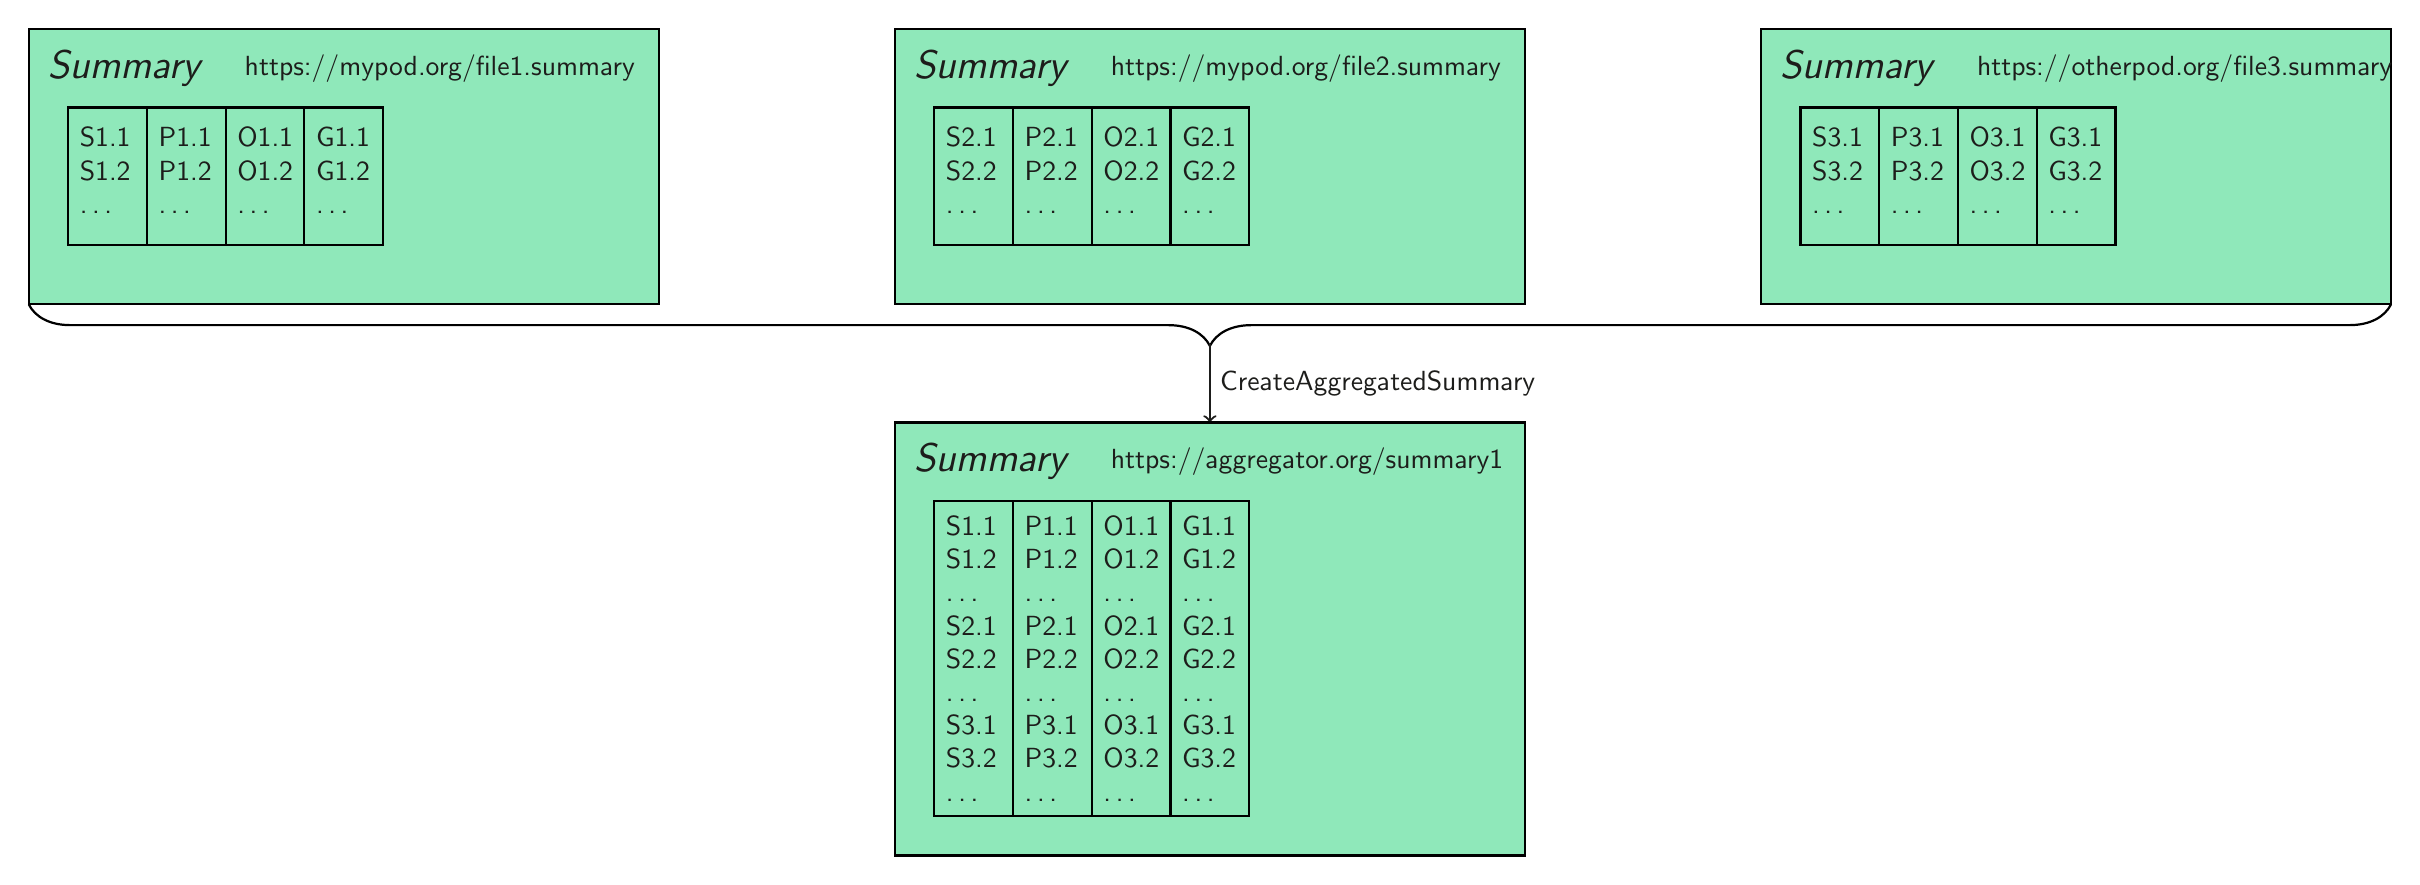
\begin{tikzpicture}[
    node distance = 10em, auto, thick,
    title/.style={text=colortext,font={\Large\itshape}},
    person/.style={text=colorwhite,font={\Large\bfseries}},
    code/.style={text=colortext,font={}},
    key/.style={text=colorkey,font={\tiny\itshape}}
]
    % Summary 1
    \draw[fill=colorsummary] (0,3) rectangle (8,-0.5);
    \node[title,text width=10em] at (2, 2.5) {Summary};
    \node[code,text width=10em] at (4.5,2.5) {https://mypod.org/file1.summary};
    
    % Components 1
    \draw[fill=colorsummary] (0.5,2) rectangle (1.5,0.25);
    \node[code,text width=2em] at (1,1.2) {S1.1\\S1.2\\\ldots};
    \draw[fill=colorsummary] (1.5,2) rectangle (2.5,0.25);
    \node[code,text width=2em] at (2,1.2) {P1.1\\P1.2\\\ldots};
    \draw[fill=colorsummary] (2.5,2) rectangle (3.5,0.25);
    \node[code,text width=2em] at (3,1.2) {O1.1\\O1.2\\\ldots};
    \draw[fill=colorsummary] (3.5,2) rectangle (4.5,0.25);
    \node[code,text width=2em] at (4,1.2) {G1.1\\G1.2\\\ldots};

    
    % Summary 2
    \draw[fill=colorsummary] (11,3) rectangle (19,-0.5);
    \node[title,text width=10em] at (13, 2.5) {Summary};
    \node[code,text width=10em] at (15.5,2.5) {https://mypod.org/file2.summary};
    
    % Components 2
    \draw[fill=colorsummary] (11.5,2) rectangle (12.5,0.25);
    \node[code,text width=2em] at (12,1.2) {S2.1\\S2.2\\\ldots};
    \draw[fill=colorsummary] (12.5,2) rectangle (13.5,0.25);
    \node[code,text width=2em] at (13,1.2) {P2.1\\P2.2\\\ldots};
    \draw[fill=colorsummary] (13.5,2) rectangle (14.5,0.25);
    \node[code,text width=2em] at (14,1.2) {O2.1\\O2.2\\\ldots};
    \draw[fill=colorsummary] (14.5,2) rectangle (15.5,0.25);
    \node[code,text width=2em] at (15,1.2) {G2.1\\G2.2\\\ldots};
    
    
    % Summary 3
    \draw[fill=colorsummary] (22,3) rectangle (30,-0.5);
    \node[title,text width=10em] at (24, 2.5) {Summary};
    \node[code,text width=10em] at (26.5,2.5) {https://otherpod.org/file3.summary};
    
    % Components 3
    \draw[fill=colorsummary] (22.5,2) rectangle (23.5,0.25);
    \node[code,text width=2em] at (23,1.2) {S3.1\\S3.2\\\ldots};
    \draw[fill=colorsummary] (23.5,2) rectangle (24.5,0.25);
    \node[code,text width=2em] at (24,1.2) {P3.1\\P3.2\\\ldots};
    \draw[fill=colorsummary] (24.5,2) rectangle (25.5,0.25);
    \node[code,text width=2em] at (25,1.2) {O3.1\\O3.2\\\ldots};
    \draw[fill=colorsummary] (25.5,2) rectangle (26.5,0.25);
    \node[code,text width=2em] at (26,1.2) {G3.1\\G3.2\\\ldots};
    
    % Aggregation
    \draw [decorate,decoration={brace,amplitude=15pt,mirror}] (0,-0.5) -- (30,-0.5);% node [code,midway,yshift=-28pt] {CreateAggregatedSummary};

    % Arrows
    \draw[->,thick,colortext] (15,-1) -- (15,-2) node[midway] {CreateAggregatedSummary};
    
    % Summary Agg
    \draw[fill=colorsummary] (11,-2) rectangle (19,-7.5);
    \node[title,text width=10em] at (13, -2.5) {Summary};
    \node[code,text width=10em] at (15.5,-2.5) {https://aggregator.org/summary1};
    
    % Components Agg
    \draw[fill=colorsummary] (11.5,-3) rectangle (12.5,-7);
    \node[code,text width=2em] at (12,-5) {S1.1\\S1.2\\\ldots\\S2.1\\S2.2\\\ldots\\S3.1\\S3.2\\\ldots};
    \draw[fill=colorsummary] (12.5,-3) rectangle (13.5,-7);
    \node[code,text width=2em] at (13,-5) {P1.1\\P1.2\\\ldots\\P2.1\\P2.2\\\ldots\\P3.1\\P3.2\\\ldots};
    \draw[fill=colorsummary] (13.5,-3) rectangle (14.5,-7);
    \node[code,text width=2em] at (14,-5) {O1.1\\O1.2\\\ldots\\O2.1\\O2.2\\\ldots\\O3.1\\O3.2\\\ldots};
    \draw[fill=colorsummary] (14.5,-3) rectangle (15.5,-7);
    \node[code,text width=2em] at (15,-5) {G1.1\\G1.2\\\ldots\\G2.1\\G2.2\\\ldots\\G3.1\\G3.2\\\ldots};

\end{tikzpicture}
\end{document}
